\section{Processi casuali stazionari}
%FIXME non è chiaro
In generale è definito processo casuale\index{Processo casuale (PC)}\footnote{Può essere definito anche un segnale casuale} -PC- un esperimento casuale il cui esito è una funzione nel tempo $y(t)$. Questa funzione prende il nome di realizzazione. Nel corso di questa trattazione verranno considerati solo PC a tempo discreto rappresentati con un indice temporale intero.\newline
Un PC possiamo immaginarlo come un vettore di VC di lunghezza infinita, dove la posizione nel vettore corrisponde all'indice temporale, quindi per un tempo fissato $\bar{t}$, $y(\bar{t})$ corrisponde ad una singola VC. I PC che andiamo a considerare in questa trattazione sono quelli stazionari\index{Processo casuale stazionario}. Un PC si dice stazionario se per un qualsiasi numero $n$ di campioni scelti nel PC $t_1, ...t_n$, le proprietà statistiche non cambiano per un qualunque sfasamento temporale $\tau$ rispetto ai campioni originali\footnote{In altre parole le VC corrispondenti ad istanti diversi del processo casuale devono avere tutte la stessa ddp}.

\subsection{Media del primo ordine}
In generale $m_y(t)=E[y(t)]$ è una funzione del tempo $t$; occupandoci solo di processi stazionari, questo non è più vero, infatti, risulta $m_y(t)=m_y$. Se dipendesse dal tempo, violerebbe l'invarianza alle traslazioni temporali e quindi non può essere definito un PC stazionario.\newline
Per un PC stazionario è facile calcolare la $m_y$: basta calcolare la media campionaria del segnale $y(t)$.\newline 
A volte può essere utile studiare i PC stazionari con media nulla; possiamo ricondurre un qualsiasi PC stazionario a media non nulla in uno a media nulla. Considerando $\tilde{y}(t)=y(t)-m_y$ risulta che $E[\tilde{y}(t)]=0$; in questo modo ci siamo ricondatti ad un PC stazionario $\tilde{y}(t)$ a media nulla.\newline
%FIXME non mi è chiara l'ergodicità
Parliamo di processi ergodici\index{Ergodicità}... \textbf{[non mi è chiara l'ergodicità]}
\subsection{Covarianza ed autocovarianza}
Prima di introdurre la funzione di autocovarianza vediamo la funzione di covarianza, di cui l'autocovarianza è un caso particolare. La covarianza\index{Covarianza} $cov(X,Y)$ di due VC $X$,$Y$ è un indice di come le due VC variano assieme, in pratica è un indicatore di indipendenza; difatti se la covarianza è nulla $cov(X,Y)=0$ le due VC sono indipendenti. Il calcolo della covarianza è definito come:

  \[ cov(X,Y)=E\left[(X-E[X])(Y-E[Y])\right]=E[XY]-E[X]E[Y] \]
La covarianza gode delle seguenti proprietà:

  \begin{align*}
    cov(X,Y)&=cov(Y,X)\\
    cov(aX+b,Y)&=acov(X,Y)\\
    cov(X+Y,Z)&=cov(X,Z)+cov(Y,Z)
  \end{align*}

L'autocovarianza\index{Autocovarianza} è la covarianza su uno stesso segnale rispetto ad uno sfasamento temporale. Siano dati due istanti $t_1$,$t_2$ e il PC $x(t)$, definiamo l'autocovarianza come:
  \begin{align*}
    \gamma_{xx}(t_1,t_2)&=E\left[(x(t_1)-E[x(t_1)])(x(t_2)-E[x(t_2)])\right]\\
       \gamma_{xx}(\tau)&=E[(x(t)-E[x(t)])(x(t+\tau)-E[x(t)])] \quad \tau=t_1-t_2
  \end{align*}
Trattando PC stazionari, $E[x(t)]=m_x$ e quindi:

  \[ \gamma_{xx}(\tau)=E[(x(t)-m_x)(x(t+\tau)-m_x)] \]

\noindent L'autocovarianza ha le seguenti proprietà:

  \begin{align*}
    \gamma_{yy}(t_1,t_2)&=\gamma_{yy}(t_2,t_1)\\
          \gamma_{yy}(0)&=Var[y(t)]
  \end{align*}
        
% ########################################################################
% ########################################################################
\paragraph{Rumore Bianco - White Noise - WN}
Il rumore bianco\index{Rumore bianco}\index{White noise} è un particolare segnale che ha la caratteristica di essere totalmente incorrelato. Quindi $x(t)$ è $WN$ se $x(t_1)$ e $x(t_2)$ sono incorrelate $\forall \quad t_1\neq t_2$, ovvero: 

\[ \gamma_{xx}(t_1,t_2)=0 \quad t_1 \neq t_2 \Longrightarrow \text{PC stazionario}\quad \gamma_{xx}(\tau)=0 \quad r\neq 0 \]

\begin{figure}[htbp]
  \centering
  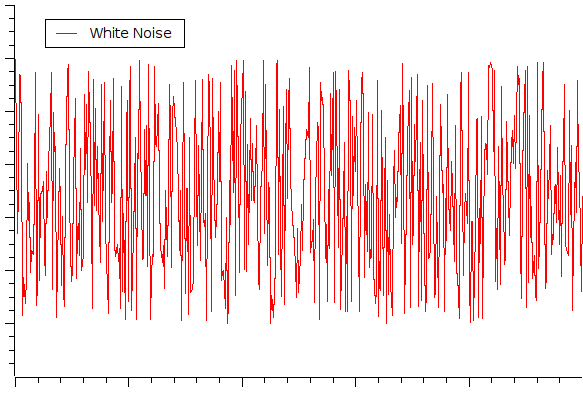
\includegraphics[scale=1]{mathematica/whitenoise}
  \caption{Andamento del segnale white noise\label{fig:WN}}
\end{figure}

\noindent Un segnale di tipo WN, rappresentato in figura \ref{fig:WN}, viene indicato con:

\[x(t)\sim WN(m_x,\sigma_X^2) \]

Se due eventi $x(t_1)$ e $x(t_2)$ sono indipendenti si dice che $x(t)$ è un WN in senso stretto. Concludiamo con l'osservazione che un segnale WN è impredicibile, è il tipo di processo casuale più casuale che possa esistere, quindi è impossibile estrarre informazioni da un segnale di questo tipo.
